\chapter{Versuchsaufbau}

\section{Einleitung}

Um die vom Team erstellte Plattform auch unter realen Bedingungen testen zu können, wurde ein Versuchsaufbau mit zwei Drohnen erstellt, welche es ermöglichen Produkte zu transportieren und über dem Kunden mit einem Fallschirm abzuwerfen. Der Aufbau der Drohnen beinhaltete die Zusammenstellung der passenden Komponenten, den Zusammenbau der Drohnen und die Planung und Erstellung von zusätzlichen Halterungen für die obengenannten spezifischen Anforderungen.\\

\subsection{Kommunikationshardware}
\label{sec:communication-hardware}
Da die Drohne eine Verbindung zum Server benötigt, muss geeignete Kommunikationshardware installiert werden. Aus folgenden Gründen haben wir uns für ein Android-Smartphone entschieden:
\begin{itemize}
	\item{Der Status der Drohne und Anweisungen zur Beladung können angezeigt werden}
	\item{Die Anbindung an den Flight-Controller ist über eine bestehende API möglich}
	\item{Das Android-Betriebssystem stellt die Kommunikation über WLAN oder GSM zur Verfügung}
\end{itemize}

Falls die Beladung automatisiert wird, oder keine Beladung notwendig ist, benötigt man nicht zwingend ein Smartphone. Um Gewicht und Platz auf der Drohne zu sparen gibt es folgende Alternativen:
\begin{itemize}
	\item{\textbf{Raspberry PI} \\
	Bereits ab dem leichtgewichtigen Raspberry PI zero sind die nötigen Funktionen vorhanden. Zusätzlich muss hier auf ein GSM Modem zurückgegriffen werden um eine permanente Internetverbindung aufzubauen. Bei Verwendung eines Raspberry PI 3 kann sogar auf ein eingebautes WLAN Interface verwendet werden.
	}
	\item{\textbf{Arduino} \\
	Bei der Arduino Hardware Plattform kann auf einem beliebigen Arduino Board implementiert werden, welches als USB Host Device arbeiten kann. Zusätzlich muss ein GSM Shield 2 verwendet werden um eine GSM Verbindung aufbauen zu können. Eine Option auf WLAN existiert nur durch zusätzliche Komponenten.}

	\item{\textbf{Pixhawk Controller mit GSM Modul} \\
	Es existieren GSM Module, wie etwa DroneCell \cite{drone-cell}, die am Pixhawk angeschlossen werden können. Diese ersetzen die Funkverbindung und ermöglichen die Kommunikation über 4G.
	}

\end{itemize}

Die ersten zwei Alternativen benötigen zusätzlich eine externe Stromversorgung. Somit muss ein \Gls{BEC} (Battery Eliminator Circuit) verwendet werden um eine stabile Spannung für die jeweilige Komponente zu liefern. \\


\section{Ablieferungskonzept}
\label{chap:ablieferung}
Um ein möglichst sicheres und einfaches Ablieferungsverfahren zu finden, wurden folgende Optionen in Betracht gezogen.

\subsection{Landung ohne automatischen Abwurf}

Bei diesem Konzept landet die Drohne an der Position des Kunden und dieser kann dann selbst das Paket von der Drohne lösen. Er wird dann mit Hilfe der Onboard-App aufgefordert den Erhalt der Bestellung zu bestätigen. Nach der Bestätigung startet die Drohne einen Countdown, hebt danach ab und fliegt zur Ausgangsposition zurück. Der Kunde kann den Countdown unterbrechen und erneut starten.

Vorteile:
\begin{itemize}
	\item Kunde bestätigt Lieferung
	\item Ware kann keinen Schaden nehmen
	\item Kunde kann entscheiden wann es sicher genug ist, damit die Drohne starten kann.
	\item Die Lieferung ist punktgenau
\end{itemize}


Nachteile:
\begin{itemize}
	\item Drohne kann Personen verletzen, während sie sich in Bodennähe befindet
	\item Aufwendiges Handling auf der Onboard-App
	\item Landung kann je nach Gelände schwierig sein
	\item Fremde Personen haben physischen Zugriff auf die Drohne
\end{itemize}

\subsection{Landung mit automatischem Abwurf}

Dieses System ermöglicht es ohne Fallschirm die Ware abzuwerfen. Dabei Landet die Drohne, löst die Ladung und startet sofort wieder. Es gibt keinerlei Interaktion mit dem Kunden.

Vorteile:
\begin{itemize}
	\item Ware kann keinen Schaden nehmen
\end{itemize}


Nachteile:
\begin{itemize}
	\item Drohne kann Personen verletzen, während sie sich in Bodennähe befindet
	\item Landung kann schwierig sein je nach Gelände
	\item Fremde Personen haben physischen Zugriff auf die Drohne
\end{itemize}


\subsection{Abwurf mit Fallschirm}

Dabei wird ein Fallschirm an der Ware befestigt. Die Drohne löst die Ladung in einer vorgegebenen Höhe und die Ladung schwebt zu Boden.

Vorteile:
\begin{itemize}
	\item Drohne kann niemanden Verletzen
	\item Drohne ist ausser Reichweite von Personen
	\item Einfaches Handling auf der Onboard-App
	\item Mechanismus erlaubt auch Landung mit automatischem Abwurf
\end{itemize}


Nachteile:
\begin{itemize}
	\item Ware kann Schaden nehmen
	\item Ware kann Personen verletzen bei Versagen des Fallschirms
	\item Einweg-Fallschirme (Kosten und Abfall)
	\item Windlage kann Fallschirm-Flugrichtung beeinflussen
\end{itemize}


\subsection{Entscheidung}

\begin{figure}[H]
	\centering
	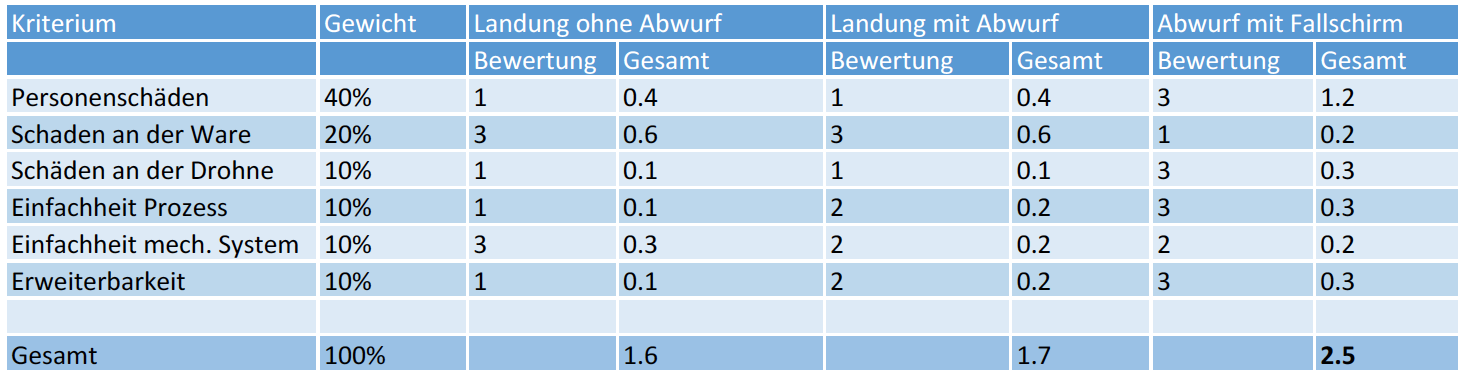
\includegraphics[width=0.9\textwidth] {images/nutzwertanalyse_abwurf.png}
	\caption{Nutzwertanalyse der verschiedenen Liefervarianten}
	\label{fig:nutzwertanalyse_abwurf}
\end{figure}


Die Nutzwertanalyse in Abbildung \ref{fig:nutzwertanalyse_abwurf} zeigt klar, dass die letzte Variante die meisten Vorteile bringt. Wichtig ist auch, dass ein Abwurf im gelandeten Zustand weiterhin möglich bleibt, ohne die mechanischen Komponenten zu verändern. Deshalb haben wir uns für einen Abwurf mit dem Fallschirm entschieden.

\subsection{Fallschirmgrösse}

Für den Fallschirm musste die optimale Grösse berechnet werden. Aufgrund der Resultate aus dem Tragfähigkeitstests (Kapitel \ref{sec:drone-gewichttest}) wird die Grösse für eine $1/2$-Liter Flasche berechnet.
Eine PET-Flasche die von einem ein Meter hohen Tisch (h) fällt, bleibt unbeschädigt. Aus diesem Grund haben wir die Geschwindigkeit für diesen Aufprall errechnet.

\begin{equation}
\label{eq:pet}
\begin{split}
v &= \sqrt{2gh} \\
v &= \sqrt{2 \cdot 9.81\frac{\text{m}}{\text{s}^2} \cdot 1.0\text{m}} \\
v &= 4.429 \frac{\text{m}}{\text{s}} \approx 4.5 \frac{\text{m}}{\text{s}} \\
\end{split}
\end{equation}

Nun musste der Fallschirm dimensioniert werden.
\begin{figure}[H]
	\centering
	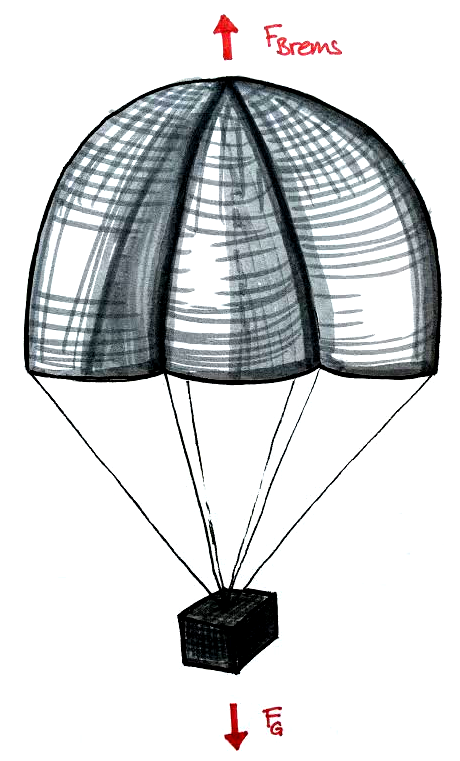
\includegraphics[width=0.3\textwidth] {images/fallschirm_berechnung.png}
	\caption{Skizze des physikalischen Modells eines Fallschirms}
	\label{fig:fallschirm-berechnung}
\end{figure}
Einfachheitshalber wird angenommen, dass der Fallschirm die Form einer Kugelkalotte, wie dies in der Grafik \ref{fig:fallschirm-berechnung} dargestellt, hat und ein Zielgewicht von 500g. Die Fläche des Fallschirms kann anhand der folgender Gleichung ausgedrückt werden:


\begin{equation}
\begin{split}
F_{\text{Brems}} &= F_{\text{G}} \\
c_{w} \cdot A \cdot \frac{\rho}{2} \cdot v_{\text{sink}}^{2} &= m_{\text{Pet}} \cdot g \\
A &= \frac{2 \cdot m_{\text{Pet}} \cdot g}{\rho \cdot c_{w} \cdot v_{\text{sink}}^{2} } \\
\end{split}
\end{equation}

Nun lässt sich der Durchmesser ($d$) über die Öffnungsfläche $A = \pi \cdot r^2$ berechnen. Wir näheren an, dass der Öffnungsdurchmesser dem Fallschirmdurchmesser entspricht.

\begin{equation}
\begin{split}
\pi \cdot r^2 &= \frac{2 \cdot m_{\text{Pet}} \cdot g}{\rho \cdot c_{w} \cdot v_{\text{sink}}^{2} } \\
r &= \sqrt{\frac{2 \cdot m_{\text{Pet}} \cdot g}{\rho \cdot c_{w} \cdot v_{\text{sink}}^{2} \cdot \pi}} \\
d &= 2 \cdot \sqrt{\frac{2 \cdot m_{\text{Pet}} \cdot g}{\rho \cdot c_{w} \cdot v_{\text{sink}}^{2} \cdot \pi}} \\
\end{split}
\end{equation}

Für die Luftdichte $\rho$ wurde der Standardwert von $1.225 \frac{\text{kg}}{\text{m}^{3}}$ genommen. Für den Strömungswiderstandskoeffizenten $c_w$ wird vom Literaturwert für die konkave Seite der Halbkugelschale abgesehen und der Erfahrungswert\footnote{Herr Prof. Dr. F. Müller hat uns darauf hingewiesen, dass aus seinen Raketenversuchen ein $c_w$-Wert von $1.80$ als gute Annäherung verwendet werden kann.} $1.80$ verwendet.
\begin{equation}
\begin{split}
d &= 2 \cdot \sqrt{\frac{2 \cdot 0.5\text{kg} \cdot  9.81\frac{\text{m}}{\text{s}^2}}{1.225 \frac{\text{kg}}{\text{m}^3} \cdot 1.80 \cdot 4.5 \frac{\text{m}}{\text{s}} \cdot \pi}} \\
d &= 1.12\text{m} \\
\end{split}
\end{equation}
Der Durchmesser des Prototypenfallschirms muss somit etwa $1.12 \text{m}$ betragen.

\newpage
\section{Multicopter Hardware}

Bei der Zusammenstellung der Komponenten haben wir vor allem auf die gute Verfügbarkeit von
Ersatzteilen und einen hohen Marktanteil der Komponenten geachtet. Besonders wichtig erschien uns, dass ein Anbieter nicht an einen Hersteller gebunden ist, sondern die Drohne an seine Bedürfnisse (Zuladung, Reichweite, Geschwindigkeit) anpassen kann. Es sollten also möglichst wenige Voraussetzungen bestehen um die Plattform nutzen zu können. Folgende Anforderungen sind allerdings unabdingbar:
\begin{itemize}
	\item Flight-Controller muss \Gls{MAVLink} Protokoll unterstüzen
	\item Onboard-App muss über MAVLink mit dem Flight-Controller verbunden sein. (Über USB oder eine Funk-Telemetrieverbindung.)
\end{itemize}

\subsection{Teile-Liste}

\begin{tabularx}{\textwidth}{|X|l|l r|}
	\hline
	\textbf{Bezeichnung} & \textbf{Bezugsquelle} && \textbf{Preis}\\
	\hline \hline
	DJI F450 ARF Kit & conrad.ch & CHF &229.95 \\\hline
	DJI F450/F550 Landegestell & conrad.ch & CHF &24.95 \\\hline
	3DR Pixhawk & 3dr.com & USD& 199.99 \\\hline
	3DR uBlox GPS with Compass Kit & 3dr.com & USD &89.99 \\\hline
	Pixhawk external LED and USB & 3dr.com & USD & 20.00 \\\hline
	FrSky X8+ Radio Transmitter & 3dr.com & USD & 89.99 \\\hline
	FrSky X8R Receiver & hebu-shop.ch & CHF & 39.95 \\\hline
	Delock Micro USB OTG Kabel & digitec.ch & CHF &15.90 \\\hline
	Multistar High Capacity 4S Akku (2x) & hobbyking.com & USD& 50.50 \\\hline
	APM Flight Controller Damping Platform & hobbyking.com & USD& 2.69 \\\hline
	Smartphone und GPS Halterung & eigener 3D-Print & CHF &27.50\\\hline
	Abwurfvorrichtung & eigener 3D-Print & CHF &25.50\\\hline
	Hitec Super Servo S-Bec (Stromversorgung Servo) & brack.ch & CHF &13.90\\\hline
	Tactic TSX10 (Servo für Abwurf) & brack.ch & CHF & 14.90\\\hline
	Kleinmaterial & diverse & CHF & 50.00\\\hline
	\hline
	\textbf{Total} & & \textbf{CHF/USD} & $\boldsymbol{\approx 900.00}$\\\hline
\end{tabularx}\\

Es wurde ein Wechselkurs von 1:1 angenommen.

\subsection{Frame und Antrieb}

Der Frame, die Motoren und ESCs wurden als Kit gekauft. Es handelt sich dabei um ein DJI Flamewheel 450 Frame mit DJI 2312 960kV Motoren und ESeries 420 20A ESCs. Dieses Kit ist weltweit gut verfügbar und deshalb ideal geeignet um einen Versuchsaufbau zu erstellen.

\begin{figure}[h]
	\centering
	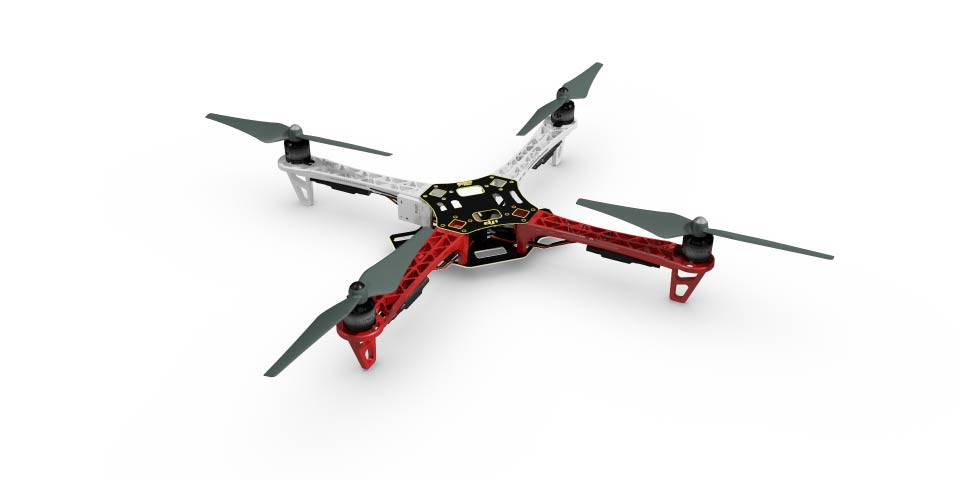
\includegraphics[width=0.9\textwidth] {images/hardware/f450.jpg}
	\caption{DJI F450 Flamewheel Kit}
	\label{fig:f450}
\end{figure}


\subsection{Flight-Controller}

Der Flight-Controller ist das Herzstück eines Multicopters. Im Unterschied zu anderen ferngesteuerten Fahr- und Flugzeugen kann ein Multicopter nur über ein Fly-by-Wire System kontrolliert werden. Das heisst alle Befehle, die von der Fernbedienung gesendet werden, müssen interpretiert und umgewandelt werden, damit die Motoren eine Bewegung in die gewünschte Richtung erzeugen können. In Kombination mit einem GPS Modul (Abb. \ref{fig:gps-module}) ermöglich der Controller verschiedene Flugmodi, wie beispielsweise das Schweben an einem Punkt oder automatisches Abfliegen von Wegpunkten.

Als Flight-Controller setzen wir ein Pixhawk ein. Es ist sehr vielseitig und kann gut mit zusätzlichen Sensoren erweitert werden, ausserdem unterstützt es gängige Firmwares, die auch auf günstigeren Controllern laufen. Als Firmware für das Pixhawk setzen wir ArduCopter ein, da sie komplett Open-Source ist und auch bei vielen anderen Projekten eingesetzt wird. Sie unterstützt ausserdem das \Gls{MAVLink} Protokoll.

\begin{figure}[h]
	\centering
	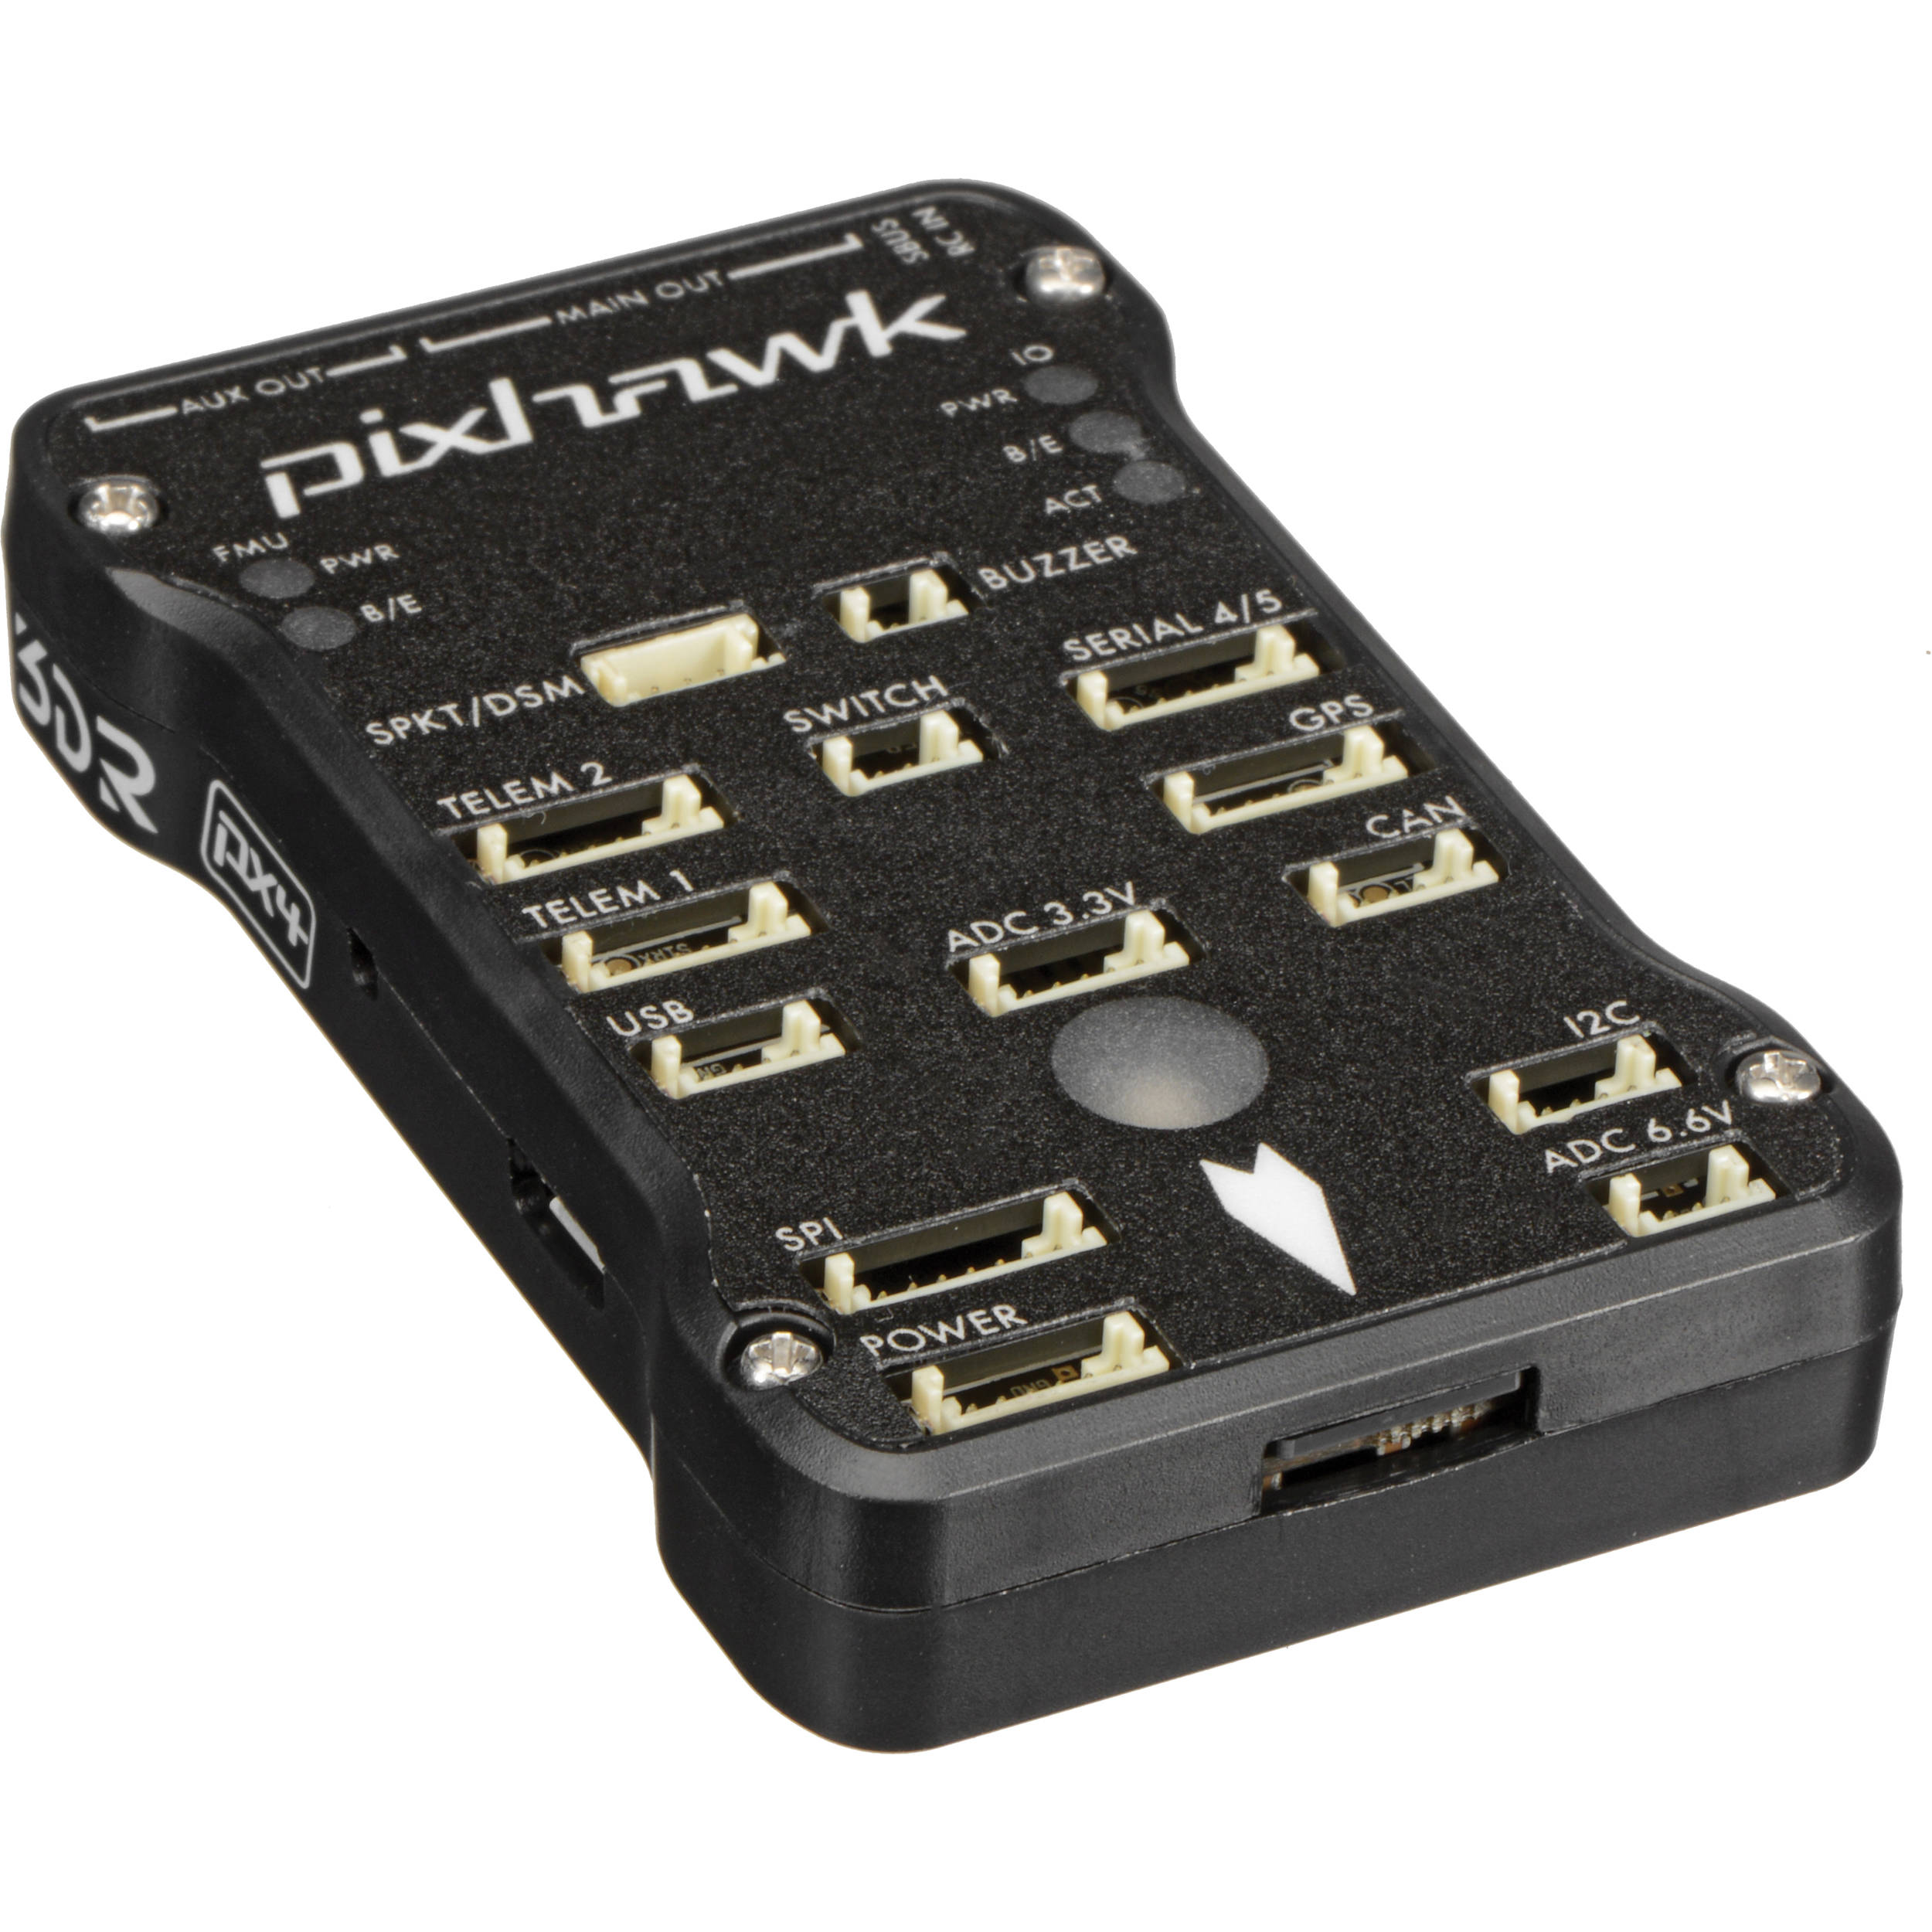
\includegraphics[width=0.3\textwidth] {images/hardware/pixhawk.jpg}
	\caption{Pixhawk Flight-Controller}
	\label{fig:pixhawk}
\end{figure}

\begin{figure}[h]
	\centering
	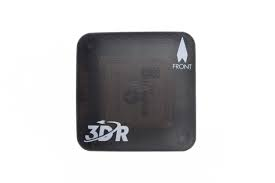
\includegraphics[width=0.3\textwidth] {images/hardware/gps-module.jpg}
	\caption{GPS-Modul für Pixhawk}
	\label{fig:gps-module}
\end{figure}

\subsection{Ausbaustufen}

Während des Projekts wurde die Hardware laufend den Bedürfnissen angepasst. Daher sind mehrere Versionen der Drohne entstanden, die für die Versuche genutzt wurden und halfen Risiken früh auszuschliessen.

\subsubsection{Version 1}

\begin{figure}[H]
	\centering
	\includegraphics[width=1.0\textwidth] {images/hardware/prototype1.jpg}
	\caption{Erster Prototyp ohne Landegestell und ohne Smartphone}
	\label{fig:prototyp-1}
\end{figure}

Um das Zusammenspiel der Hardwarekomponenten zu testen und erste Erfahrungen mit dem GPS und den verschiedenen Flugmodi zu sammeln, wurde in der ersten Iteration nur die Drohne in einem minimal Flugzustand aufgebaut.

\subsubsection{Version 2}

\begin{figure}[H]
	\centering
	\includegraphics[width=1.0\textwidth] {images/hardware/prototype2.jpg}
	\caption{Drohnen Aufbau mit Smartphone}
	\label{fig:prototyp-2}
\end{figure}

Um die Risiken R08 (Ardupilot Handhabung) und R09 (Ardupilot API) frühzeitig auszuschliessen (siehe Tabelle \ref{table:risk-table}), wurde das Smartphone provisorisch auf die Drohne montiert, und mit einem ersten Prototypen der Onboard-App getestet. \\
Nach dem Test wurde uns klar, dass eine Befestigung für das Smartphone erarbeitet werden musste, um es sicher zu transportieren und bedienbar zu positionieren.

\begin{figure}[H]
	\centering
	\begin{minipage}[b]{0.4\textwidth}
		% TODO Ein Bild ohne Tastatur und Stuhl wäre auch gut?
		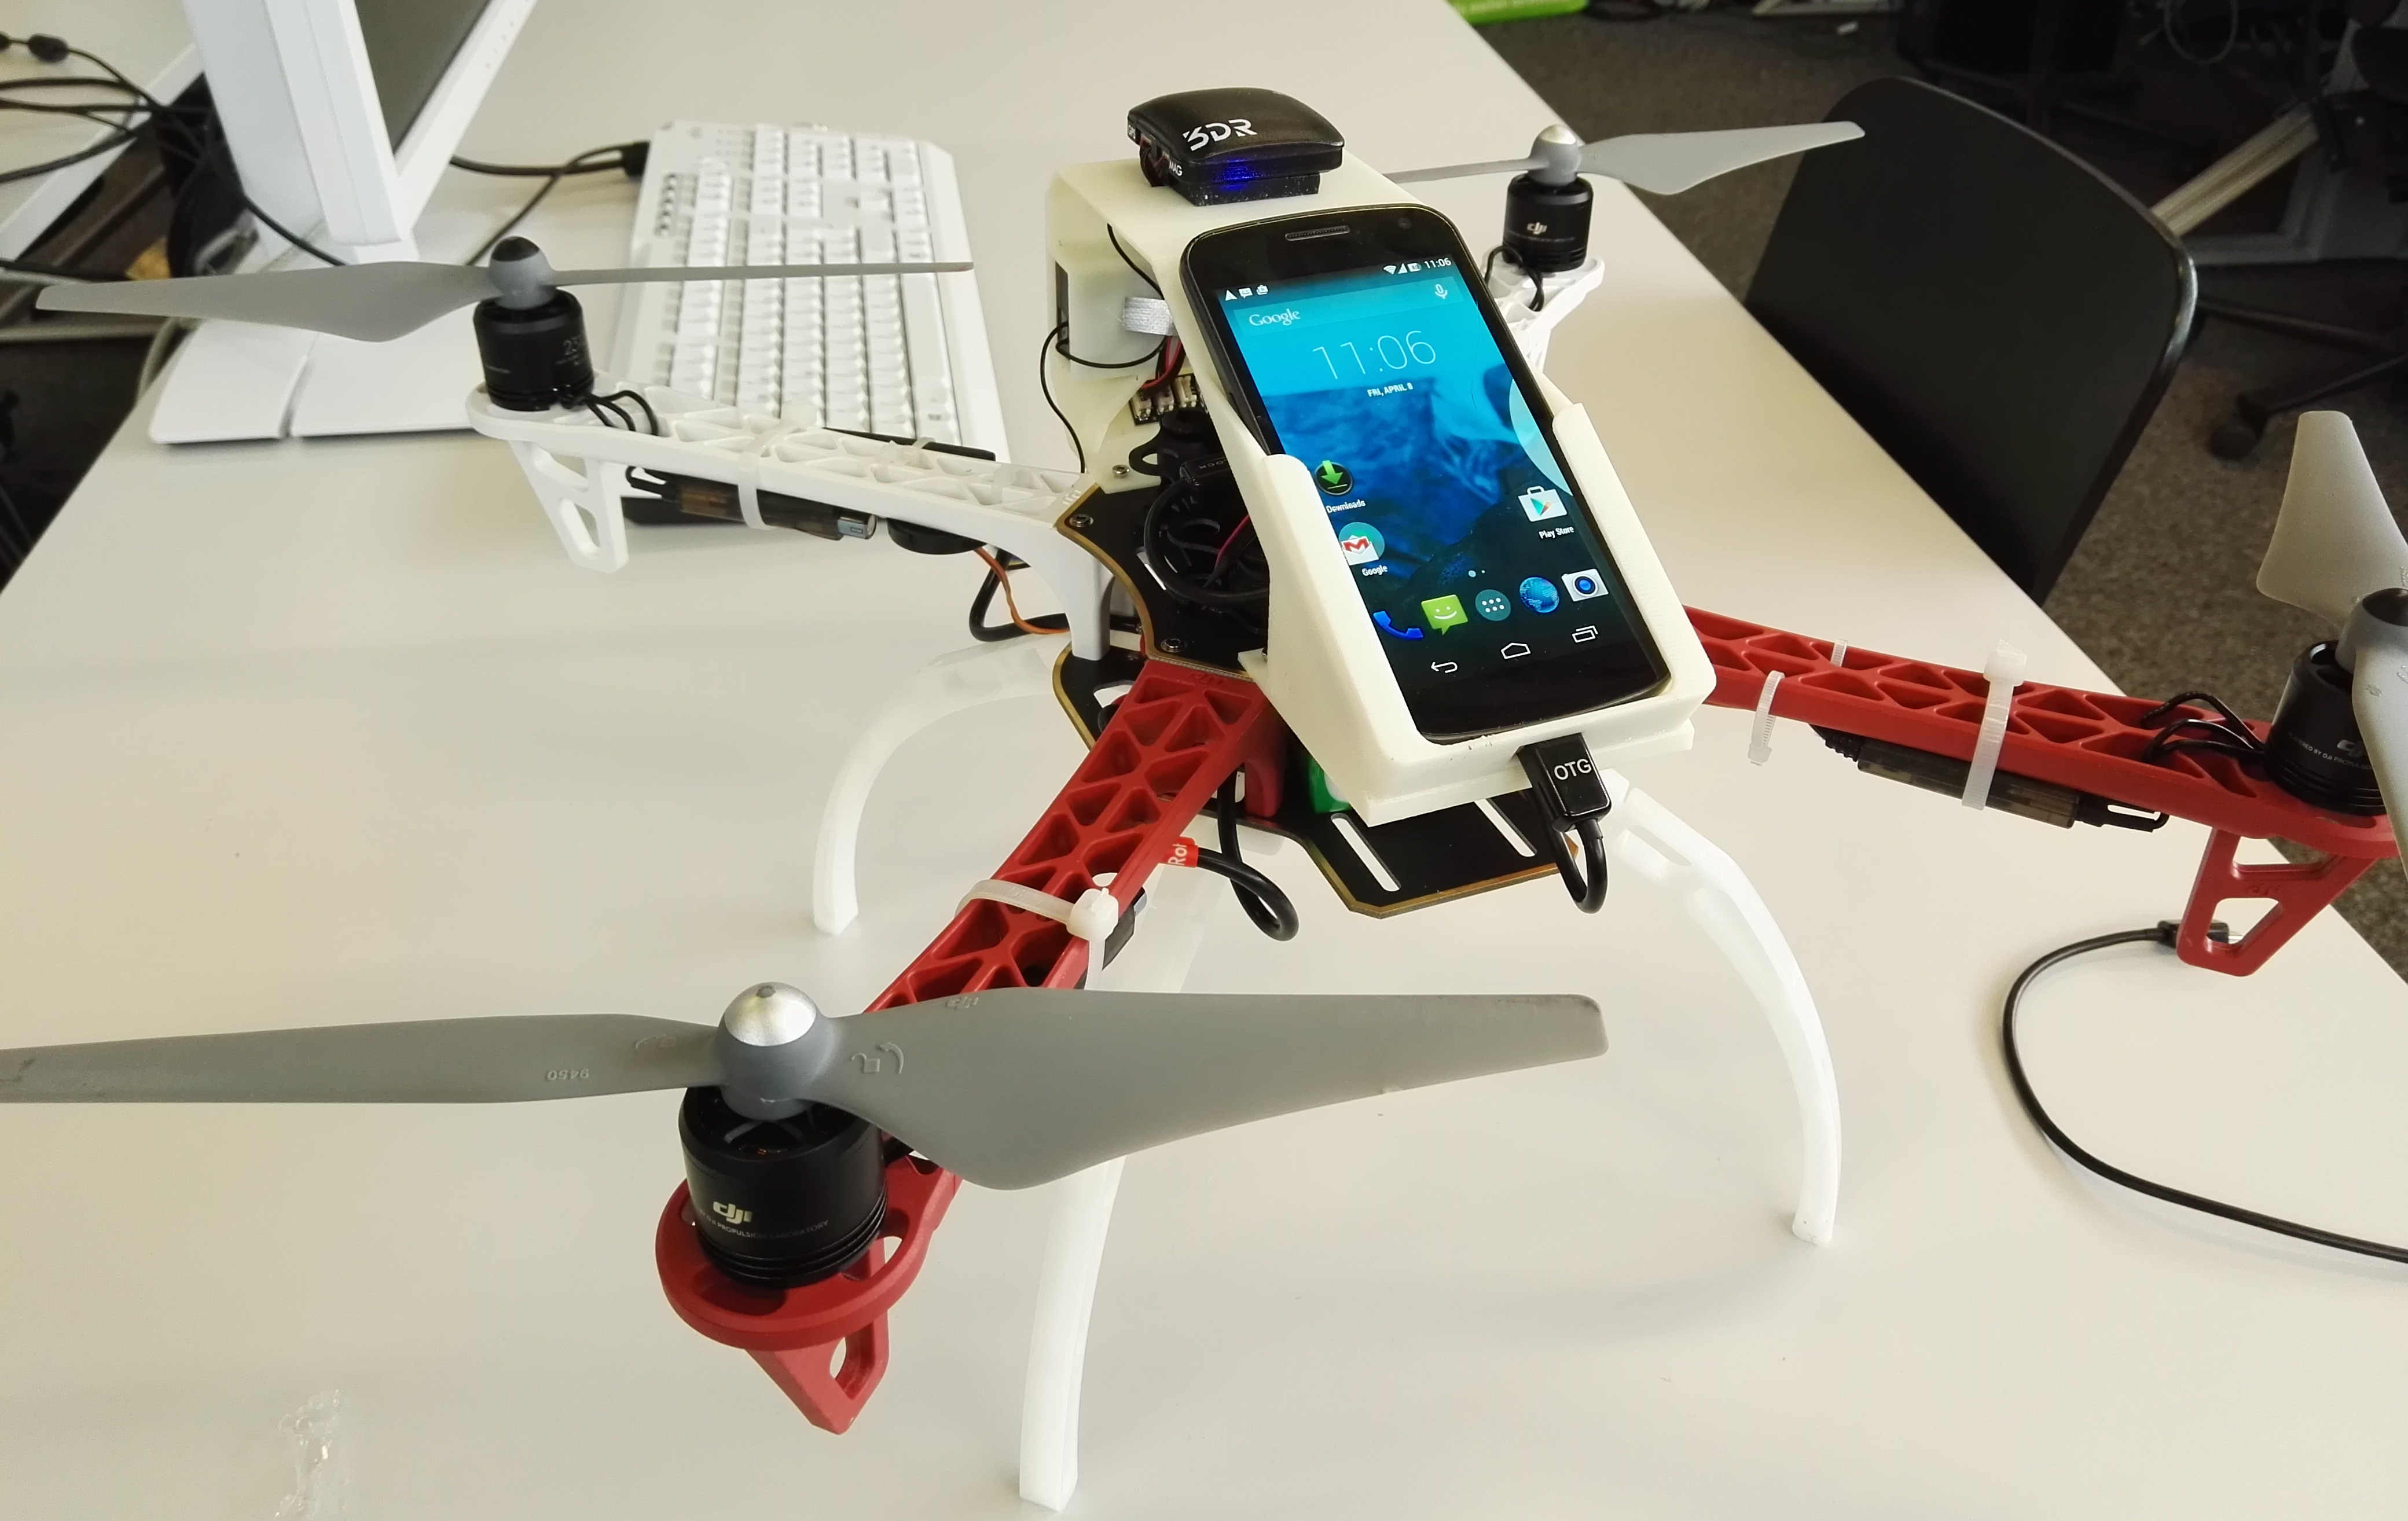
\includegraphics[width=\textwidth]{images/hardware/drone-with-handy.jpg}
		\caption{Drohne mit Handy Halterung}
		\label{fig:prototyp-3}
	\end{minipage}
	\hfill
	\begin{minipage}[b]{0.4\textwidth}
		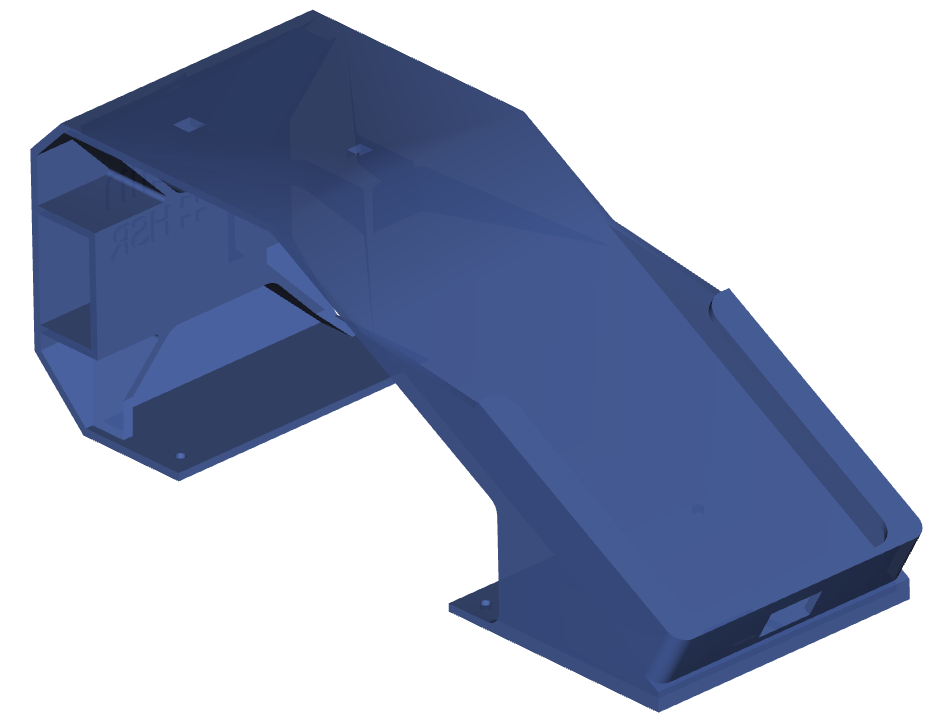
\includegraphics[width=\textwidth]{images/hardware/case-model.png}
		\caption{3D-Modell der Handy Halterung}
		\label{fig:case-model}
	\end{minipage}
\end{figure}

Es wurde eine Halterung konzipiert (siehe Abb.\ref{fig:case-model}), welche wir im 3D-Druck Verfahren produzieren liessen.
Die Handy-Halterung konnte auch gleich genutzt werden, um das GPS-Modul an einer passenden Stelle zu positionieren.

\subsubsection{Version 3}
Nachdem mit der Drohne zahlreiche autonome Testflüge unternommen wurden, musste eine Möglichkeit erarbeitet werden, wie die Lieferung an den Kunden gebracht werden kann ( Abschnitt \ref{chap:ablieferung} ).

\begin{figure}[H]
	\centering
	\begin{minipage}[b]{0.4\textwidth}
		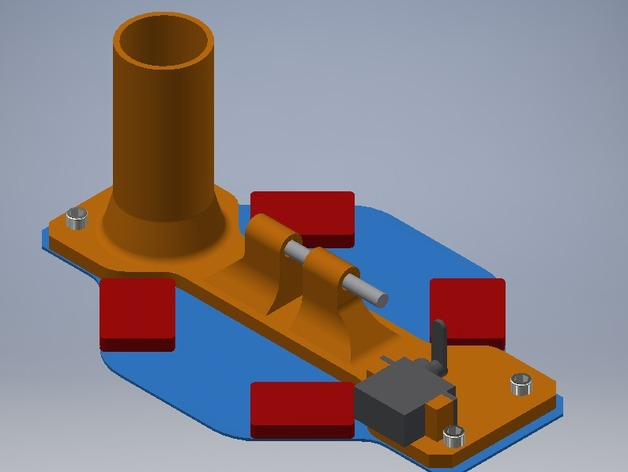
\includegraphics[width=\textwidth]{images/hardware/parachute-model.jpg}
		\caption{Halterung}
		\label{fig:parachute-mode}
	\end{minipage}
	\hfill
	\begin{minipage}[b]{0.4\textwidth}
		% TODO Hier muss ein bessers Bild her ( oder Kafferahmen weg photoshoppen )
		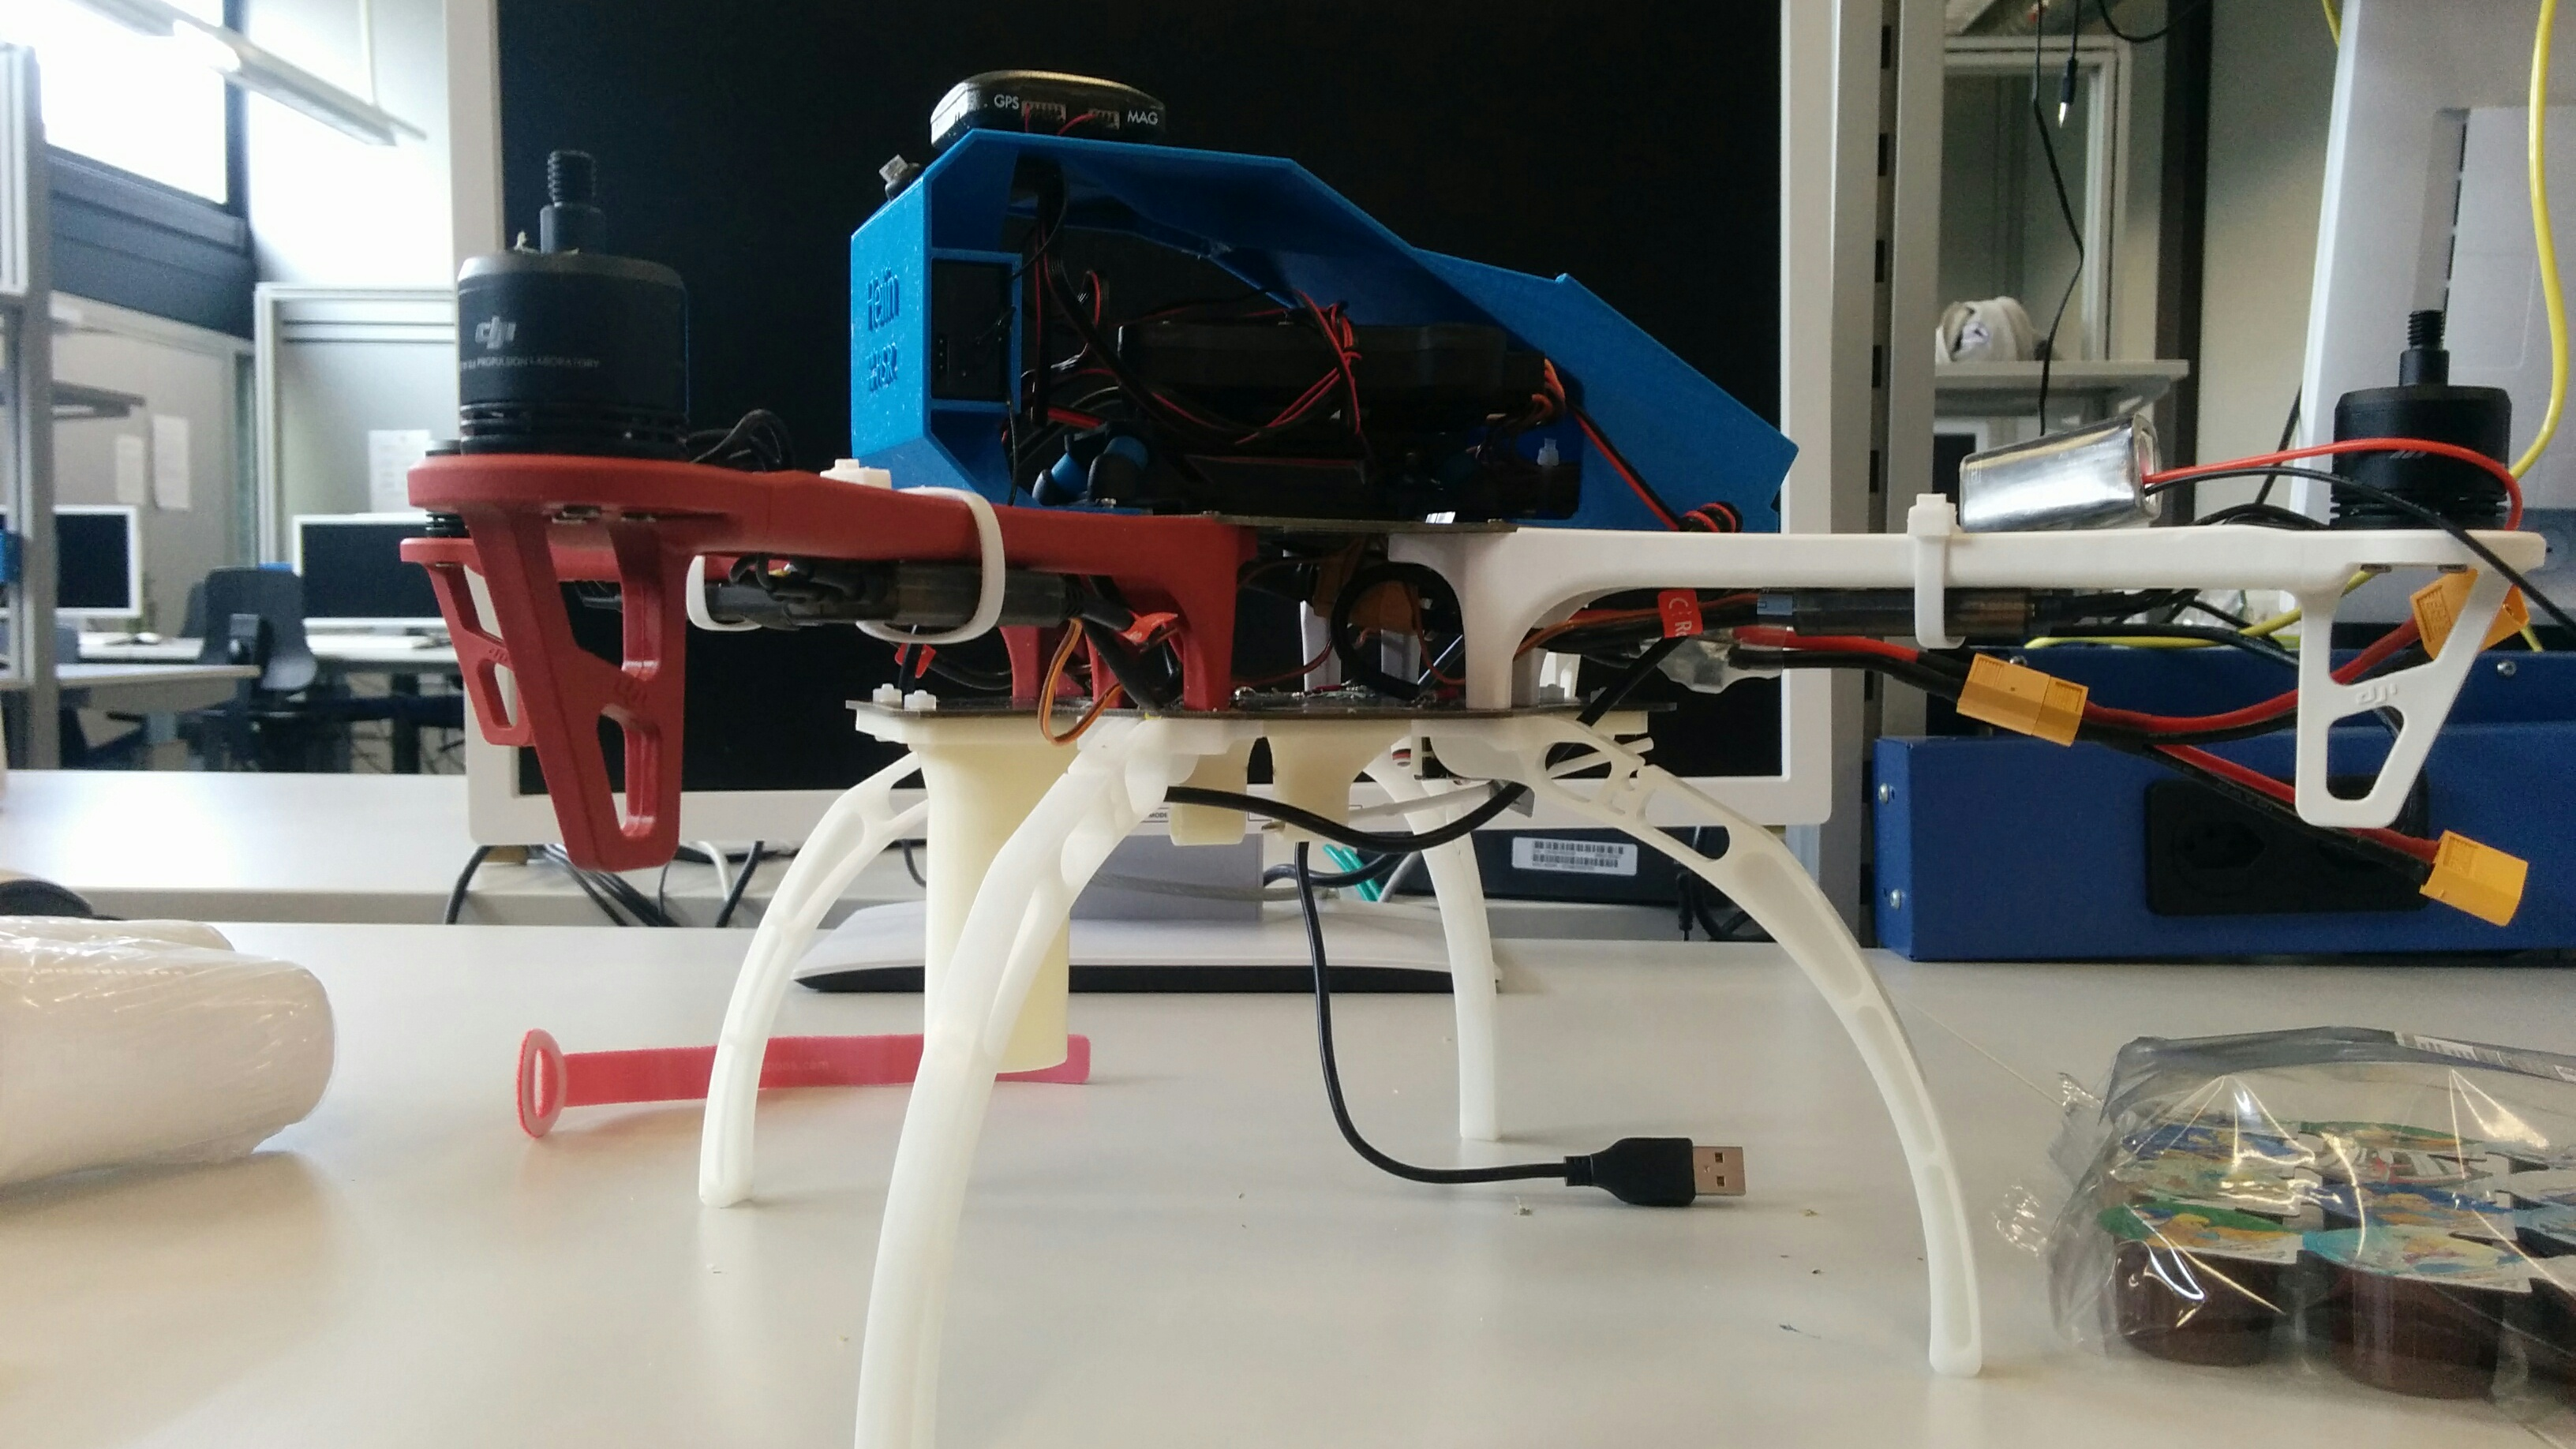
\includegraphics[width=\textwidth]{images/hardware/drone-with-servo.jpg}
		\caption{Drohne mit dem Abwurfsmechanismus}
		\label{fig:drone-with-servo}
	\end{minipage}
\end{figure}


Es wurde ein einfacher Mechanismus mit einem handelsüblichen Modelbau-Servo konstruiert. Die Abbildung \ref{fig:drone-with-servo} zeigt, den Mechanismus mit dem Stift, der vom Servo herausgezogen werden kann. Das Rohr auf der Vorrichtung dient zur Aufbewahrung des Fallschirms während des Flugs. Nach dem Lösen des Stifts zieht das Gewicht der Ladung den Fallschirm aus dem Rohr.\\

\subsection{Tests}
Um die Anwendungsmöglichkeiten eines solchen Multicopters auszuloten wurden diverse Experimente durchgeführt um die Leistungsfähigkeit und die Einschränkungen zu testen.

\subsubsection{Akku Laufzeittest}
Um die maximale Akku Laufzeit zu testen wurde die Drohne ohne zusätzliches Gewicht gestartet, etwa 1.5m über dem Boden schweben gelassen und die Zeit gemessen. Dabei versucht die Drohne die Postion zu halten, bei Abweichung wurde aktiv korrigiert. \\

\begin{tabularx}{\textwidth}{|c|c|X|}
	\hline
	\textbf{Akku} & \textbf{Zuladung} & \textbf{Laufzeit} \\ \hline \hline
	3S & keine & 16min 29s\\ \hline
	2x 4S & 500g & 19min\\ \hline
\end{tabularx}

\subsubsection{Tragfähigkeitstests}
\label{sec:drone-gewichttest}

Um das maximale Gewicht zu prüfen, welches auf unsere Drohnen geladen werden kann, wurden Tests mit dem Zielgewicht von ca. 500g durchgeführt. Dies Entspricht dem Gewicht einer $1/2$-Liter Flasche oder einem leichten Defibrilator. Ausserdem war das Mobiltelefon (ca. 150g) während des Tests auf der Drohne angebracht.  \\

\begin{tabularx}{\textwidth}{|c|c|c|c|X|}
	\hline
	\textbf{Nutzlast} & \textbf{Akku Typ} & \textbf{Nötige Leistung }& \textbf{Erwartete Flugzeit } & \textbf{Subjektives Flugverhalten }\\
	\hline \hline
	500g & 3S & ca. 75\%  & n.A. & Ziemlich Träge, mehr Gewicht wäre kritisch\\\hline
	500g & 4S & ca. 45\%  & n.A. & Gewicht kaum Spürbar\\
	\hline
\end{tabularx}\\

Auch mit 3S Akkus ist es also möglich eine PET-Flasche zu transportieren. Allerdings empfehlen wir für Gewichte über 300 Gramm 4S-Akkus zu verwenden.\\

Aus den Tragfähigkeitstests schliessen wir, dass auch ein Defibrillator (siehe Aufgabenstellung) mit einer von uns erstellten Drohne transportierbar ist. Folgende Textpassage \cite[p.3]{FleckUAV} bestätigt, dass in einem ähnlichen Gewichtsbereich bereits Produkte existieren.

\blockquote{I identified the two lightest weight defibrillators on the market in the U.S. at the time of the exploration (March 2013): the Schiller FRED EasyPort (600 grams) and the HeartSine samaritan PAD 300P (1100 grams). The former model is not designed for layperson use, but is far and away the lightest defibrillator available.}



\newpage

\section{Alternative Drohnenarten}
\label{sec:drone-alternatives}

Grundsätzlich können, über das von uns verwendete \Gls{MAVLink} Protokoll, alle Arten von Drohnen angesteuert werden. Wie in Abbildung \ref{fig:arduScreenshot} ersichtlich, bietet die Autopilot-Software 'ArduPilot' Varianten für Multicopter, Flugzeuge und Fahrzeuge an.\\
\begin{figure}[H]
\centering
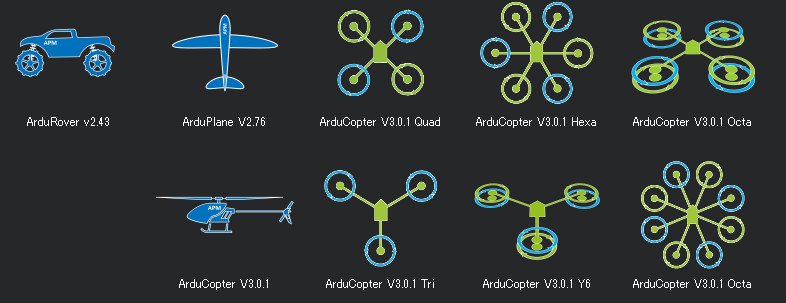
\includegraphics[width=0.8\textwidth] {images/arduScreenshot.jpg}
\caption{Screenshot der verschiedenen Firmwarevarianten.}
\label{fig:arduScreenshot}
\end{figure}

\begin{figure}[H]
	\centering
	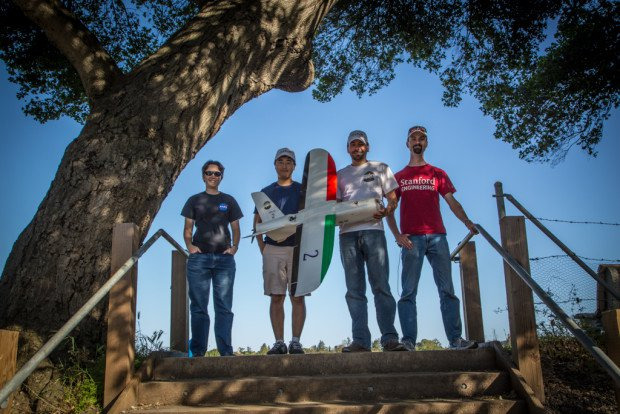
\includegraphics[width=0.8\textwidth] {images/SyriaUplift.jpg}
	\caption{Uplift Team und die Syrien-Drohne Quelle: \protect\url{http://uplift.aero/}}
	\label{fig:uplift}
\end{figure}

Auch andere Projekte könnten von unserem System profititeren. Uplift Aero beispielsweise, ist ein Startup, dass Hilfsgüter mit Hilfe von Drohnen von der Türkei aus nach Syrien fliegen wollte. Sie haben für ihre Flugzeuge (Grafik \ref{fig:uplift}) die selben Flugcontroller wie wir verwendet, mussten lediglich eine andere Firmware aufspielen. Dies beweist wie flexibel und vielseitig die von uns eingesetzte Hardware verwendet werden kann.






